% !TEX root = ../../../main.tex
% 来源：中学数学实验教材·第二册（几何）
% 章节：轨迹与作图 / 作图
% 原始文件：5.tex，行 469-482
% 类型：tikz
% ---
    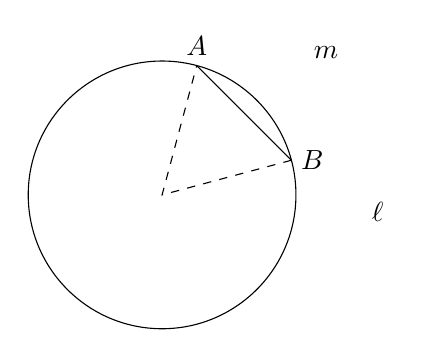
\begin{tikzpicture}[>=latex, scale=1.7]
\draw (0,0) circle(1);
\tkzDefPoints{0/0/O}
\tkzDrawPoints(O)
\tkzLabelPoints[below](O)
\tkzDefPoint(-5:1){C}
\tkzDefPoint(45:1){D}
\tkzDrawLines[add=.5 and .5](O,C O,D)
\draw[dashed](15:1)node[right]{$B$}--(0,0)--(75:1)node[above]{$A$};
\draw (75:1)--(15:1);
\node at (-5:1.5)[right]{$\ell$};
\node at (45:1.5)[right]{$m$};

    \end{tikzpicture}
